\documentclass{article}
\usepackage[italian]{babel}
\usepackage[tmargin=2cm,rmargin=1.5in,lmargin=1.5in,margin=0.85in,bmargin=2cm,footskip=.2in]{geometry}
\usepackage{siunitx}
\sisetup{separate-uncertainty=true, per-mode=fraction, parse-numbers=true}
\usepackage{caption}
\usepackage[T1]{fontenc}
\usepackage{bookmark}
\usepackage{graphicx}
\usepackage{multicol}
\usepackage{booktabs}
\usepackage{amsmath,amsfonts,amsthm,amssymb,mathtools}
\hypersetup{
	pdftitle={Appunti Tomadin},
	colorlinks=true, linkcolor=doc!90,
	bookmarksnumbered=true,
	bookmarksopen=true
}
\usepackage{blindtext}
\usepackage{wrapfig}
\usepackage{listings}
\usepackage{xcolor}
\usepackage{float}
\usepackage{tikz}
\usepackage{multirow}
\usepackage{biblatex}
\definecolor{codegreen}{rgb}{0,0.6,0}
\definecolor{codegray}{rgb}{0.5,0.5,0.5}
\definecolor{codepurple}{rgb}{0.58,0,0.82}
\definecolor{backcolour}{rgb}{0.95,0.95,0.92}
\definecolor{doc}{rgb}{0,0,0}
\lstdefinestyle{code}{
    backgroundcolor=\color{backcolour},   
    commentstyle=\color{codegreen},
    keywordstyle=\color{magenta},
    numberstyle=\tiny\color{codegray},
    stringstyle=\color{codepurple},
    basicstyle=\ttfamily\footnotesize,
    breakatwhitespace=false,         
    breaklines=true,                 
    captionpos=b,                    
    keepspaces=true,                                     
    showspaces=false,                
    showstringspaces=false,
    showtabs=false,                  
    tabsize=2,
    inputencoding=ansinew,
    extendedchars=true,
    numbers=left,                    
    numbersep=5pt
}

\lstset{style=code}
\usepackage[varbb]{newpxmath}
\usepackage{circuitikz}
\title{Relazione sui rimbalzi di una pallina}
\author{Aiello Giosuè, Fenili Domenico, Sermi Francesco}
\date{\today}

\begin{document}
\maketitle
\pagebreak
\tableofcontents
\pagebreak
\section{Scopo dell'esperienza}
Determinare la validità del modello teorico scelto per una pallina che cade rimbalzando su una superficie rigida
\section{Premesse teoriche}
Nel modello più semplice ipotizzabile per una pallina che cade rimbalzando, possiamo supporre che questa perda una frazione $\gamma$ indipendentemente dalla velocità posseduta prima della caduta. Se lasciamo cadere quindi una pallina da un'altezza nota $h_0$ con velocità iniziale nulla:
\begin{equation}
	h_n = h_0 \gamma ^n
\end{equation}
dove $n$ rappresenta il numero di rimbalzi. In questo modello è facilmente dimostrabile che l'altezza massima raggiungibile può essere determinata partendo dai tempi di rimbalzo con la seguente formula, sebbene non tenga conto di effetti come la resistenza dell'aria:
\begin{equation}
	h_n = \frac{1}{8} g (t_n - t_{n-1})^2
\end{equation}
\section{Strumenti e materiali}
Per effettuare questa esperienza abbiamo utilizzato i seguenti materiali:
\begin{itemize}
	\item una pallina da tennis elastica;
	\item un metro a nastro
\end{itemize}
Per quanto riguarda gli strumenti abbiamo invece utilizzato:
\begin{itemize}
	\item \textbf{Audacity}, software per l'elaborazione dei file audio;
	\item uno smartphone, per registrare dei file audio;
\end{itemize}
\section{Descrizione sulle misure}
Prima di iniziare l'esperimento, abbiamo effettuato una serie di test per determinare l'altezza ottimale $h_0$ da cui far cadere la pallina. Questo perché, a seconda del materiale con cui è fatta, la pallina perde una quantità diversa di energia cinetica ad ogni urto, influenzando il numero di rimbalzi che possiamo registrare. Questi test preliminari ci hanno anche aiutato a trovare la posizione migliore per posizionare lo smartphone per rilevare efficacemente la pressione sonora generata dagli urti della pallina sul pavimento. Questo sarà particolarmente utile durante l'analisi dell'audio registrato. \\
\textbf{Considerazioni}: nel nostro setup sperimentale, le potenziali fonti di errore possono derivare da urti accidentali della pallina con oggetti nelle vicinanze o da rumori di fondo che potrebbero compromettere la registrazione audio. Per mitigare questi problemi, abbiamo scelto di condurre l'esperimento in un ambiente spazioso e il più silenzioso possibile.
\begin{wrapfigure}{l}{0.6\textwidth}
	\vspace{-1cm}
	\centering
	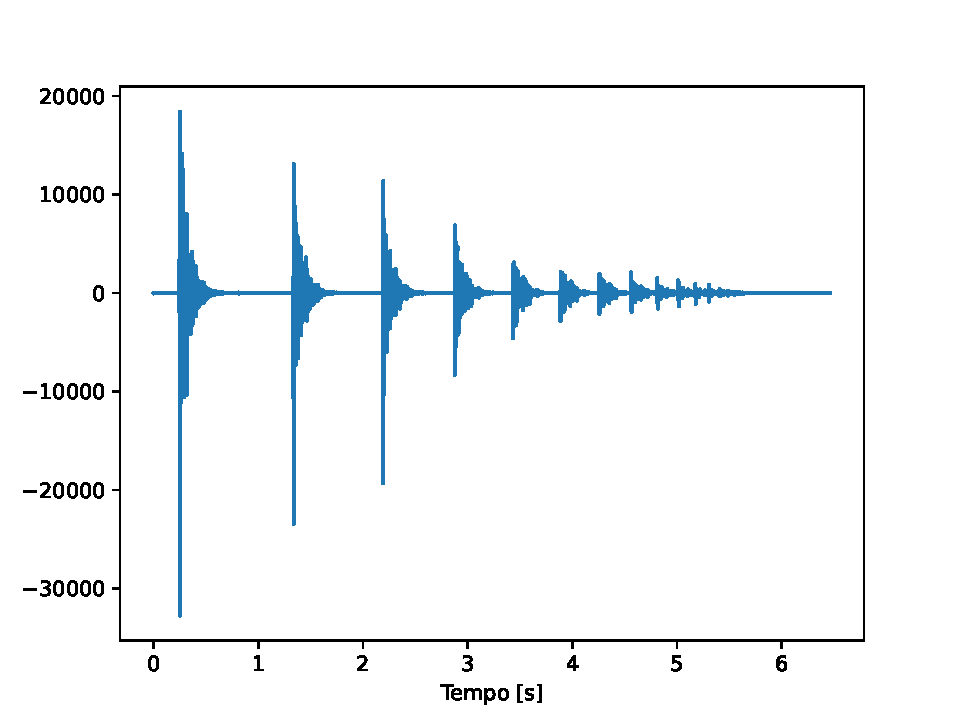
\includegraphics[width=0.3\textwidth, scale=0.1]{Grafico_rimbalzo.pdf}
	\caption{Immagine audio del campione audio misurato dal telefono: ogni rimbalzo della pallina è caratterizzato da un attacco più lungo ed una coda relativamente più lunga e già si intuisce il problema di individuare l'intervallo in cui è avvenuto l'urto}
	\label{fig:audio}
\end{wrapfigure}
\noindent Successivamente abbiamo effettuato le misure. Dopo aver raccolto il campione audio, siamo passati ad analizzarlo con la libreria \emph{matplotlib}. Non disponendo di un'applicazione per la registrazione dei suoni in grado di registrare in formato \emph{.wave} abbiamo utilizzato il software \textbf{Audacity} per convertire il file in un formato in grado di essere letto dalla libreria. \\ \\ \clearpage
\noindent La determinazione degli istanti in cui è avvenuto il rimbalzo è la fase più delicata della raccolta dati di questa esperienza e quello più soggetta agli errori accidentali e sistematici: come si può vedere dalla Figura~\ref{fig:audio} qua di lato, infatti, non è possibile individuare in maniera precisa l'\emph{esatto} istante temporale in cui è avvenuto il rimbalzo a causa della natura impulsiva delle forze che hanno agito sulla pallina.
Siccome ogni rimbalzo è caratterizzato da una serie di \emph{picchi} (fra cui è presente uno che è massimo) e una \emph{coda} abbiamo considerato come istante del rimbalzo il valore medio dell'intervallo di tempo che va dall'istante in cui la pressione sonora è massima (ovvero quando le forze impulsive sono massime) all'istante di tempo  in cui è presente un nuovo picco e come incertezza la semidispersione fra i due. \\ \\
Per fare ciò abbiamo utilizzato lo strumento \emph{Lente} presente sui grafici del file audio creati con la libreria \texttt{matplotlib}: si ingrandiva la coda dell'urto fino a posizionarci sui due picchi (quello massimo e quello successivo) col mouse e si leggeva la coordinata $x$ (ovvero il tempo) dei due riportata in alto a destra.
\noindent Successivamente, questi dati sono stati immagazzinati in un array di Python da cui poi abbiamo effettuate tutte le estrapolazioni descritte sopra. Si riporta qua sotto in tabella i dati ottenuti: \\ \\
\hspace{-0.05\textwidth} \begin{minipage}{0.5\textwidth}
	\centering
	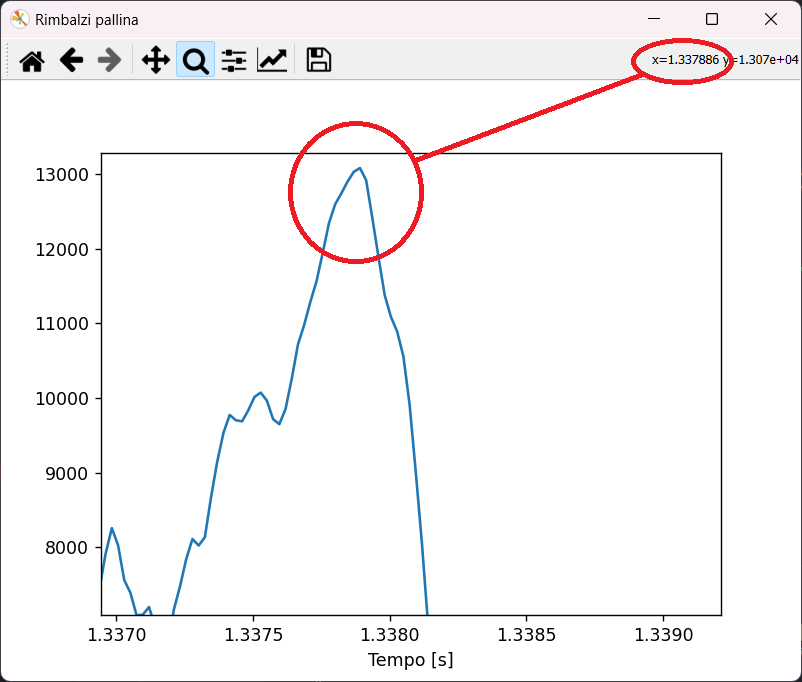
\includegraphics[scale=0.40]{Esempio_misurazione.png}
	\captionof{figure}{Immagine per chiarire come venivano effettuate le misurazioni: si ingrandiva l'immagine posizionando il cursore sul picco massimo e si leggeva il tempo in alto a destra}
\end{minipage}
\hspace{0.01\textwidth}
\begin{minipage}{0.5\textwidth}
	\centering
	\begin{tabular}{ c c }
		\toprule
		$t^*$ ($s$) & $\sigma_{t^*}$ ($s$) \\ 
		\toprule
		$0.2540$ & $0.0003$ \\ \midrule
		$1.340$ & $0.002$ \\ \midrule
		$2.195$ & $0.002$ \\ \midrule
		$2.884$ & $0.005$ \\ \midrule
		$3.440$ & $0.005$ \\ \midrule 
		$3.893$ & $0.005$ \\	 \midrule
		$4.2595$ & $0.0004$ \\ \midrule
		$4.5638$ & $0.0005$ \\ \midrule
		$4.816$ & $0.004$ \\ \midrule
		$5.017$ & $0.004$ \\ \bottomrule

	\end{tabular}
	\vspace{0.1\textwidth}
	\captionof{table}{Tabella dei tempi da noi misurati: indichiamo con $t^*$ l'istante dell'urto che abbiamo considerato essere il valore medio fra il picco massimo e il picco successivo come istante di tempo in cui è avvenuto il rimbalzo e gli abbiamo assegnato un'incertezza pari a $\sigma_t^*$ pari alla semidispersione fra i due a causa del fatto che non è possibile determinare a priori l'istante preciso in cui è avvenuto l'urto}
\end{minipage}
\section{Analisi dei dati}

Per questa analisi abbiamo utilizzato il metodo del parametro libero del fit rispetto al valore $h_0$ e il parametro $\gamma$. Abbiamo realizzato con il linguaggio di programmazione Python e la funzione \emph{curve\_fit} della libreria \emph{scipy} un grafico delle altezze $h_n$ in funzione dell'indice $n$ che rappresenta l'$n$-esimo rimbalzo della pallina. \\
Siccome il modello teorico che avevamo ipotizzato era della forma:
$$
	h_n = h_0 \gamma^n
$$
dovrebbe risultare che i nostri dati si dispongono come un esponenziale e quindi dovrebbero apparire come una retta in scala semilogaritmica. Inoltre,  tenendo $h_0$ come parametro libero, possiamo confrontare il valore stimato dal fit con quello reale per valutare di quanto si discosta dalla realtà il modello teorico. \\
Per quanto riguarda la determinazione degli errori sulle altezze, abbiamo propagato gli errori sulle altezze con la seguente formula:
$$
	\sigma_h = \frac{1}{4}g(t_n - t_{n-1})\sqrt{\sigma^2_{t_n} + \sigma^2_{t_{n-1}}}
$$
che abbiamo ottenuto considerando il fatto che gli errori relativi si sommano nel caso di prodotti e rapporti. Infatti, indicando con $\Delta t = t_n - t_{n-1}$ si deve avere che:
$$
	\frac{\sigma_{\Delta t^2}}{\Delta t^2} = 2\frac{\sigma_{\Delta t}}{\Delta t} \implies \sigma_{\Delta t^2} = 2\frac{\sigma_{\Delta t}}{\Delta t} \Delta t^{2} = 2\sigma_t \Delta t \implies \sigma_h = \frac{1}{8}g \cdot 2 \sigma_t \Delta t \implies \sigma_h = \frac{1}{4}g(t_n - t_{n-1})\sqrt{\sigma_{t_n}^2 + \sigma^2_{t_{n-1}}}
$$

\begin{wrapfigure}{l}{0.5\textwidth}
	\centering
	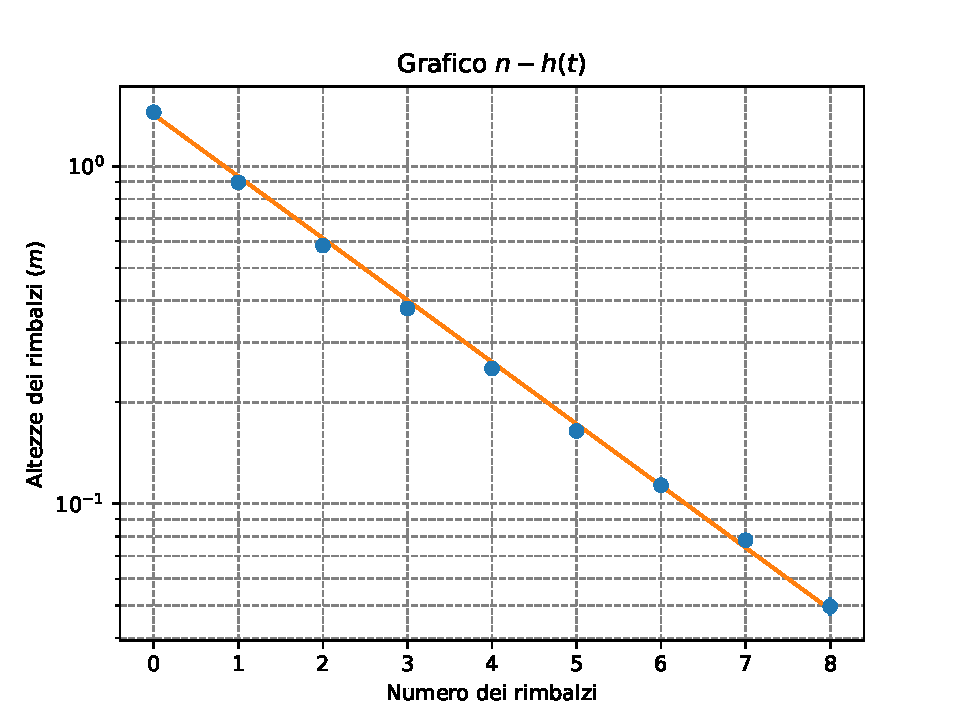
\includegraphics[scale=0.4]{Grafico_n-h(t).pdf} 
	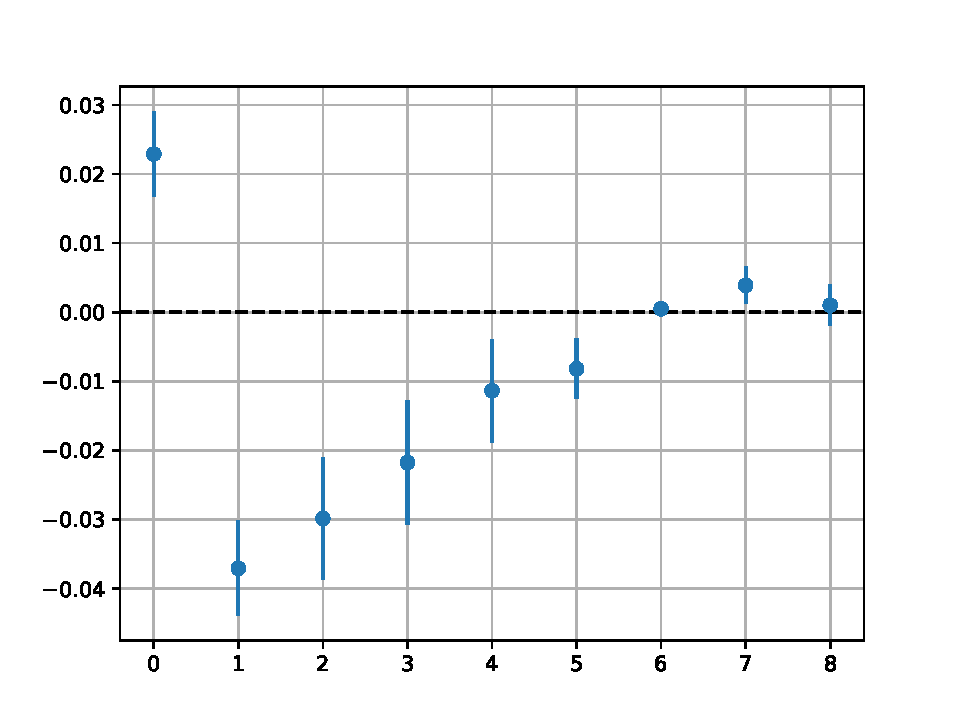
\includegraphics[scale=0.4]{Grafico_residui.pdf}
	\caption{Fit effettuato con la libreria \texttt{scipy} e grafico dei residui: sebbene il fit, ad occhio, risulti buono, si nota subito dal grafico dei residui che sono presenti sicuramente degli errori sistematici, forse dovuti al fatto che man mano che si procede con la misure gli urti diventino sempre più lunghi in senso temporale}
	\vspace{1cm}
\end{wrapfigure}

\noindent Riportiamo il fit fatto con Scipy qua di lato in scala semilogaritmica, da cui si nota (anche se non è molto visibile nell'immagine di lato), che le nostre misure non si discostano molto dal modello teorico e che il nostro modello teorico sembra effettivamente accurato. Tuttavia, la libreria \texttt{scipy} ci restituisce, tramite l'analisi per parametro libero, un altezza iniziale che denotiamo come $\hat{h_0}$ pari a:
\begin{equation}
	\hat{h_0} = (2.17 \pm 0.03) \, \text{\unit{m}}
\end{equation}
che si discosta di parecchio rispetto al valore da noi aspettato, pari a $h_0 = (2.50 \pm 0.01) \, \text{\unit{m}}$ (si parla infatti di $\approx 10.4\sigma$ di distanza). Il $\chi^2$ tuttavia risulta essere pari a
\begin{equation}
	\chi^2 \approx 69.9
\end{equation}
il che, nel nostro caso in cui abbiamo 7 gradi di libertà (9 dati sperimentali - 2 parametri da stimiamo dal fit), lascerebbe pensare che ci troviamo dinanzi ad un buon fit, sebbene i residui lascino ipotizzare la presenza di evidenti errori sistematici: infatti, se ne guardiamo il grafico, si nota che i residui non oscillano attorno allo zero, visto che alcuni di essi permangono con il segno negativo piuttosto che distribuirsi anche con segno positivo: questo indica che molto probabilmente erano presenti degli errori di natura non puramente statistica che hanno influito nelle nostre misure, pertanto il test del $\chi^2$ ci può dire ben poco visto che questo ha senso per grandezze che sono statisticamente indipendenti (e in presenza di errori sistematici ciò non è così). Si può ipotizzare che l'origine di questi errori sia probabilmente dovuta al fatto che la pallina, perdendo sempre di più energia cinetica, effettua degli urti che sono temporalmente più lunghi\footnote{infatti, si può osservare dal file audio che la pressione sonora generata dalla pallina ad ogni urto sia sempre più piccola, pertanto agiscono delle forze di modulo sempre più piccolo e che devono agire sulla pallina su tempi più lunghi per permetterle di rimbalzare} e noi, considerando solamente la distanza fra due picchi come tempo dell'urto, abbiamo sottostimato l'istante in cui il rimbalzo è avvenuto. \\ \\
Abbiamo ipotizzato, inoltre, che, oltre a quanto già espresso riguardo al fatto che man mano che la pallina effettuava degli urti via via sempre più lunghi che ci hanno fatto sottostimare l'istante effettivo del rimbalzo, l'altezza $h_0$ che avevamo preso in considerazione fosse troppo \emph{grande} e la caduta della pallina, in virtù dell'altezza, risentisse troppo della resistenza dell'aria. \\ \\
Abbiamo rifatto quindi le misurazione facendola ricadere da $h_1 = (1.50 \pm 0.01) \, \text{\unit{m}}$ di cui riportiamo le misure qua nella pagina successiva: 

\begin{wraptable}{r}{0.5\textwidth}
	\centering
	\begin{tabular}{c c}
		\toprule
		$t^*$ ($s$) & $\sigma_{t^*}$ ($s$) \\ \midrule
		$0.5484$ & $0.0005$ \\ \midrule
		$1.1012$ & $0.0005$ \\ \midrule
		$1.5470$ & $0.0005$ \\ \midrule
		$1.906$ & $0.002$ \\ \midrule
		$2.2005$ & $0.0005$ \\ \bottomrule
	\end{tabular}
	\caption{Misurazione dei rimbalzi della pallina effettuati da un'altezza minore, dove $t^*$ rimane il valore medio fra il picco massimo e il picco successivo di ogni urto e $\sigma_t^*$ la semidifferenza fra i due picchi. Uno dei problemi più grandi di queste misurazioni sono il basso numero di dati che siamo riusciti ad ottenere}
\end{wraptable}

\noindent Come si può vedere un grande problema di queste misure è il fatto che siamo stati in grado di misurare solamente 4 campioni. La libreria \texttt{scipy} anche in questo caso ha restituito un $\hat{h_1}$ totalmente diverso da quello aspettato:
\begin{equation}
	\hat{h_1} = (0.574 \pm 0.004) \unit{m}
\end{equation}
Guardando il grafico (riportato qua sotto), potremmo pensare, come prima, che i dati siano in buon accordo con il modello teorico, tuttavia, a differenza di quanto fatto prima, non possiamo dire molto  sul grafico dei residui a causa del numero esiguo di misure che siamo stati in grado di fare e anche il test del $\chi^2$ ci fa sperare ben poco riguardo alla \emph{qualità} del fit, visto che il suo valore risulta essere pari a: \\
\begin{equation}
	\chi^2 \approx 3.6
\end{equation}
che, in questo caso in cui abbiamo 2 gradi di libertà, non è un buon valore.
\\
\begin{figure}[h!]
	\centering
	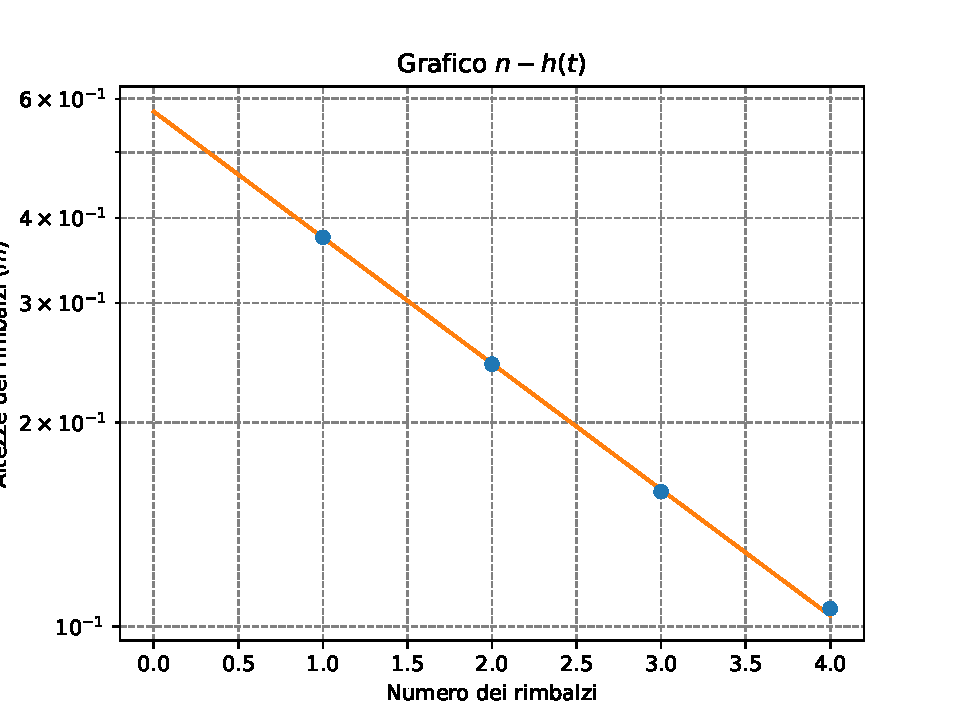
\includegraphics[scale=0.50]{Grafico_n-h(t)_(1).pdf}
	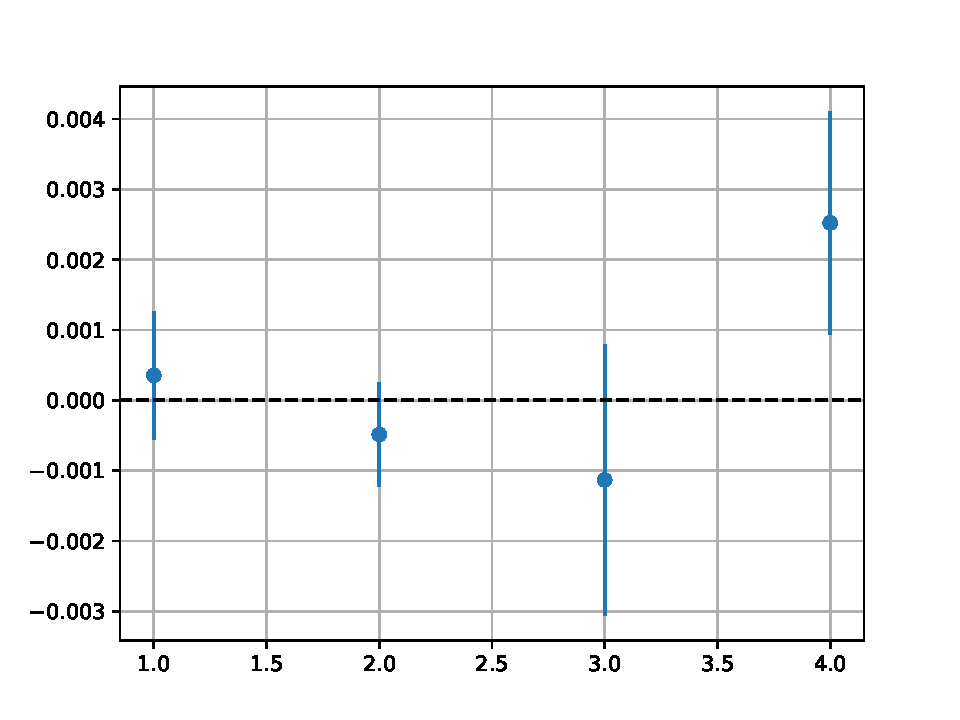
\includegraphics[scale=0.50]{Grafico_residui_(1).pdf}
	\captionof{figure}{Fit dei rimbalzi e grafico dei residui della pallina fatta cadere da un'altezza. In questo caso possiamo dire ben poco riguardo alla natura degli errori sistematici a causa del numero esiguo di misure fatte, dovuto al fatto che la pallina faceva dei rimbalzi troppo silenziosi non facilmente analizzabili con la strumentazione dai noi posseduta}
\end{figure}
\noindent Un fatto tuttavia interessante è che, in entrambe le misurazioni, se estrapoliamo attraverso il metodo del parametro libero il parametro $\gamma$, si osserva che in entrambe le misurazioni effettuate rispettivamente a $h_0$ e $h_1$ il valore ottenuto è compatibile in barre di errore. Si ha infatti che:
\begin{align*}
	&\gamma_0 = (0.656 \pm 0.002) \, \unit{\frac{J}{m}} & &\gamma_1 = (0.652 \pm 0.003) \, \unit{\frac{J}{m}}
\end{align*}
che distano in barre di errore:
$$
	\sigma = \left| \frac{\gamma_0 - \gamma_1}{\sqrt{\sigma^2_{\gamma_0} + \sigma^2_{\gamma_1}}} \right| \approx 0.6
$$
I due valori di gamma risultano quindi compatibili entro le barre di errore e potremmo quindi supporre che gli effetti che il nostro modello teorico trascura, come la resistenza dell'aria, potrebbero agire sul nostro modello come se fossero un \emph{offset} costante influenzando il moto della pallina come se fosse partita da un'altezza più bassa, tuttavia sono necessari degli esperimenti che non soffrono di errori sistematici come in questo caso.

\section{Conclusioni}

L'esperimento da noi compiuto, a causa degli errori non puramente statistici e ai metodi da noi usati (come il test del parametro libero tramite fit lineare, che funziona solo per grandezze statisticamente indipendenti), non ci ha consentito di verificare se ci sono dei motivi per supporre il rigetto del modello teorico da noi supposto. \\
Bisogna però osservare che il parametro $\gamma$ misurato in due altezze differenti risulta essere compatibile entro le barre di errore tuttavia, essendo ottenuto tramite analisi per parametro libero in presenza di errori sistematici, si potrebbe pensare di ideare altri esperimenti dove questi sono assenti o trascurabili per verificare se, con modelli teorici che tengono conto anche della resistenza dell'aria (che dalla estrapolazioni da noi effettuate pare agire come una sorta di offset costante), l'ipotesi che la pallina perda sempre una frazione $\gamma$ della sua energia cinetica sia corretta. 
\end{document}